\documentclass[11pt,a4paper]{ivoa}
\input tthdefs
\input gitmeta

\customcss{custom.css}

\usepackage{todonotes}
\usepackage{xifthen}
\lstloadlanguages{XML,SQL}
\lstset{flexiblecolumns=true,basicstyle=\ttfamily,belowskip=0pt}

\iftth
\newenvironment{args}%
{\begin{html}<ul>\end{html}\def\arg##1(##2){\begin{html}<li><i>\end{html}%
  ##1 \begin{html}</i>(<code>\end{html}##2\begin{html}) </code>\end{html}}}%
{\begin{html}</ul>\end{html}}

\newenvironment{examples}%
{\begin{html}<p><strong>Examples</strong></p><ul>\end{html}%
  \def\example{\begin{html}<li><code>\end{html}}%
  \def\becomes{\begin{html}</code><br/>\end{html} returns
    \begin{html}<code>\end{html}}%
  \def\done##1.{\begin{html}</code> <span class="explanation">\end{html}
    ##1
    \begin{html}</span></li>\end{html}}}%
{\begin{html}</ul>\end{html}}

\else
% definition pulled out of doc to hide it from tth (which gets confused
% by ifthenelse

\newenvironment{args}%
% this is *only* for use within a description environment
  {\hfil % let definition label stand on a line of its own.
    \def\arg##1(##2){\item {\textit{##1} (\texttt{##2})}}
    \begin{list}{$\bullet$}{\topsep=0pt\partopsep=0pt\parsep=0pt}
    }%
  {\end{list}}

\newenvironment{examples}%
  {\par\bigbreak
    \noindent\textbf{Examples} (non-normative)\nobreak\par
    \nobreak\vskip 3pt plus 1pt
    \def\example{\par\noindent}%
    \def\becomes{\ifhmode\hfil\break\fi\strut\qquad$\to$ }%
    \def\done##1.{\ifthenelse{\isempty{##1}}{\par}{%
        \hfil\break{\footnotesize\fontshape{it}\selectfont
        ##1.\par}}\vskip 4pt plus 2pt}}%
  {\relax}



\fi

\newcommand{\aaps}{Astronomy and Astrophysics Supplement}

\title{Catalogue of ADQL User Defined Functions}

% see ivoatexDoc for what group names to use here
\ivoagroup{DAL}

\author[https://wiki.ivoa.net/twiki/bin/view/IVOA/JonJuaristiCampillo]{Jon Juaristi Campillo}
\author[https://wiki.ivoa.net/twiki/bin/view/IVOA/MarkusDemleitner]{Markus Demleitner}


\editor[https://wiki.ivoa.net/twiki/bin/view/IVOA/JonJuaristiCampillo]{Jon Juaristi Campillo}

\previousversion[https://www.ivoa.net/documents/udf-catalogue/20231010]{EN-1.1}
\previousversion[https://www.ivoa.net/documents/udf-catalogue/20210310]{EN-1.0}
\previousversion[https://ivoa.net/documents/udf-catalogue/20200806/]{PEN-20200806}
\previousversion[https://ivoa.net/documents/udf-catalogue/20190925]{PEN-20190925}


\begin{document}
\begin{abstract}
The IVOA Astronomical Data Query Language (ADQL) has the extension
facility of user defined functions (UDFs).  While service operators are
free to define these as they see fit, it is clearly advantageous if
identical functionality is available under identical names in different
services.  Therefore, ADQL 2.1 has introduced the \verb|ivo_| prefix,
reserved for functions with agreed-upon semantics.  This endorsed note
contains this agreement and, via its updates, is the means of updating
it.
\end{abstract}


\section*{Conformance-related definitions}

The words ``MUST'', ``SHALL'', ``SHOULD'', ``MAY'', ``RECOMMENDED'', and
``OPTIONAL'' (in upper or lower case) used in this document are to be
interpreted as described in IETF standard RFC2119 \citep{std:RFC2119}.

The \emph{Virtual Observatory (VO)} is a
general term for a collection of federated resources that can be used
to conduct astronomical research, education, and outreach.
The \href{http://www.ivoa.net}{International
Virtual Observatory Alliance (IVOA)} is a global
collaboration of separately funded projects to develop standards and
infrastructure that enable VO applications.


\section{Introduction}

The Astronomical Data Query Language (ADQL) \citep{2008ivoa.spec.1030O}
has the notion of user defined functions (UDF).  These provide a
light-weight extension mechanism for operators of TAP services.
For instance, \citet{2016arXiv161109190T} show how they enable the
construction of HEALPix maps although ADQL~2.0 itself entirely lacks
facilities to deal with them.

In order to avoid different signatures or semantics on functions
offering identical or similar functionality,  this document defines UDFs
with names prefixed with \verb|ivo_|.  If services have functions with
this names, they must work as defined here.

In version 1.0, this note documents a consensus
on such functions where it has been
reached within other standards or in the review of this document.

In the future, where UDFs are not naturally associated with a
particular standard, they can be proposed by editing this document and
starting the Endorsed Note process \citep{2017ivoa.spec.0517G} on the
changes.  In effect, this endorsed note is the management tool for
the \verb|ivo_| ``namespace'' in ADQL user defined functions.

Note that no function given here is required to be present in a generic
TAP service (though other standards may pose such requirements; for
instance,
\verb|ivo_hashlist_has| is required by both
RegTAP and EPN-TAP).  However, if a service implements any UDF with a
name mentioned in this document, its semantics must be as specified here.

\subsection{Role within the VO Architecture}

\begin{figure}
\centering

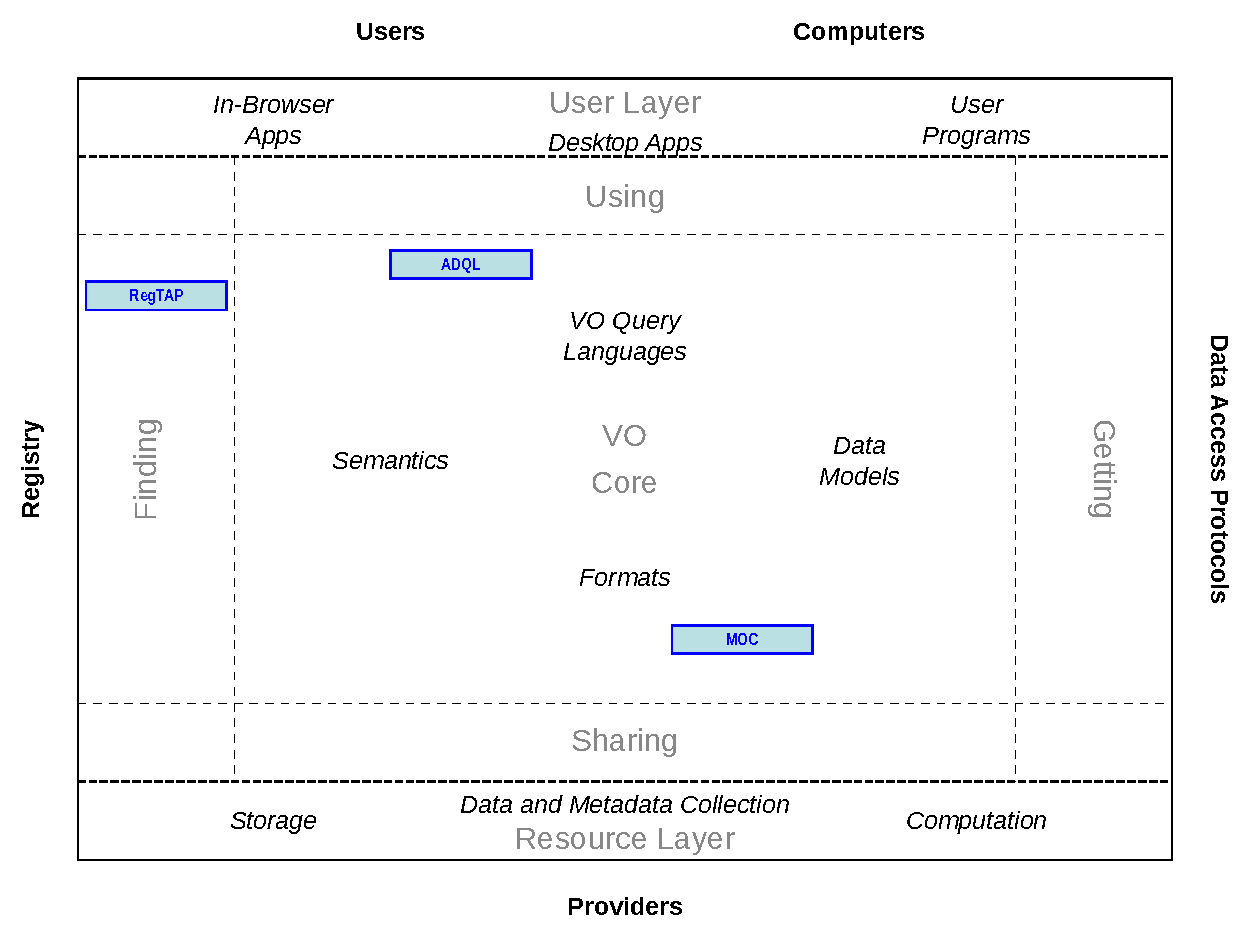
\includegraphics[width=0.9\textwidth]{role_diagram.pdf}
\caption{Architecture diagram for the UDF catalogue.}
\label{fig:archdiag}
\end{figure}

Fig.~\ref{fig:archdiag} shows the role this document plays within the
IVOA architecture \citep{2021ivoa.spec.1101D}.  It relates to the following
other standards:

\begin{bigdescription}
\item[ADQL \citep{2008ivoa.spec.1030O}] This endorsed note defines the
user defined functions with the \verb|ivo_| prefix.  While ADQL 2.0
does not treat those as special, they can be (and have been) used there
already.  Normative language on \verb|ivo_| is expected to become
part of ADQL 2.1.

\item[RegTAP \citep{2019ivoa.spec.1011D}] RegTAP first defined some of the
UDFs defined here.  It is expected that later versions of RegTAP will
refer to this note rather than maintaining a second definition, and
deferring the actual definition of UDFs to this note should be the
standard way of introducing UDFs used or required by a standard in the future.

\item[MOC \citep{2019ivoa.spec.1007F}] The HEALPix functions defined
here build on terminology introduced in the MOC specification.
\end{bigdescription}


\section{List of IVOA user defined functions}

The functions are defined through a brief human-readable description of
what the function does, followed by a closer discussion of the
parameters, the return value, and the authority the UDF was drawn from.

In the parameter definitions, we do not distinguish between different
precisions of floating point arguments.  Where we write \texttt{REAL}, the
expectation is that the functions accept floating point values of any
precision.  Similarly, we write \texttt{TEXT} for anything sufficiently
string-like, be it \texttt{CHAR(n)}, \texttt{VARCHAR(*)}, or something
comparable.

Most functions are accompanied by examples, which are intended to make
the effects of the functions clearer and give implementors a
starting point for tests.  Where examples disagree with the
specification text, the text is normative.

While ADQL does not support standalone evaluation of functions, a query
like
\begin{lstlisting}[language=SQL,aboveskip=\medskipamount]
  SELECT TOP 1 <example> AS res FROM TAP_SCHEMA.tables
\end{lstlisting}
will return one row with the function result for simple, non-aggregate
functions.


\subsection{HEALPix-related}

In this section, order and npix are used as in the Multi-Order
Coverage map (MOC) recommendation
\citep{2019ivoa.spec.1007F}.

\subsubsection{ivo\_healpix\_index(hpxOrder, long, lat)}

Returns the index (npix) of the HEALPix cell containing the spherical
point given by longitude \texttt{long} (typically, right ascension) and
latitude \texttt{lat} (typically, declination) at order
\texttt{hpxOrder} in NESTED numbering.

\begin{description}
\item[Parameters]
\begin{args}
	\arg hpxOrder (INTEGER) -- the HEALPix order to use.
	\arg long (REAL) -- longitude of the spherical point to compute the
	index for, in degrees.
	\arg lat (REAL) -- latitude of the spherical point to compute the
	index for, in degrees.
\end{args}

\item[Return type] \texttt{BIGINT}

\item[Source] This document, version 1.0
\end{description}

\begin{examples}
\example \verb|ivo_healpix_index(0, 1, 1)|
\becomes \verb|4|
\done.

\example \verb|ivo_healpix_index(17, 1, 1)|
\becomes \verb|81609757711|
\done.

\example \verb|ivo_healpix_index(17, 359, -1)|
\becomes \verb|73009064944|
\done.
\end{examples}

\subsubsection{ivo\_healpix\_index(hpxOrder, point)}

Returns the index (npix) of the HEALPix cell containing the spherical
point given by \texttt{point} at order \texttt{hpxOrder} in NESTED
numbering.

\begin{description}
\item[Parameters]
\begin{args}
	\arg hpxOrder (INTEGER) -- the HEALPix order to use.
	\arg point (POINT) -- the position to compute the index for.
\end{args}

\item[Return type] \texttt{BIGINT}

\item[Source] This document, version 1.0
\end{description}

\begin{examples}
\example \verb|ivo_healpix_index(0, POINT(1, 1))|
\becomes \verb|4|
\done.

\example \verb|ivo_healpix_index(17, POINT('ICRS', 1, 1))|
\becomes \verb|81609757711|
\done.

\example \verb|ivo_healpix_index(17, CENTROID(CIRCLE(359, -1, 3)))|
\becomes \verb|73009064944|
\done.
\end{examples}


\subsubsection{ivo\_healpix\_center(hpxOrder, hpxIndex)}

Returns a POINT corresponding to the center of the HEALPix cell
with index (npix) \texttt{hpxIndex} at order \texttt{hpxOrder} in NESTED
numbering.

\begin{description}
\item[Parameters]
\begin{args}
	\arg hpxOrder (INTEGER) -- the HEALPix order to use.
	\arg hpxIndex (INTEGER) -- the index for which to return the center
	position.
\end{args}


\item[Return type] \texttt{POINT}

\item[Source] This document, version 1.0
\end{description}

\begin{examples}
\example \verb|ivo_healpix_center(0, 6)|
\becomes \verb|[180., 0.]|
\done as a 2-array with \xmlel{xtype}=\emph{point}.

\example \verb|ivo_healpix_center(17, ivo_healpix_index(17, 23.4, 56.7))|
\becomes \verb|[23.399843462947466, 56.70016214363192]|
\done.

\example \verb|ivo_healpix_center(17, 23.2)|
\becomes undefined
\done Implementations are advised to fail when floating point numbers
are passed as indices, but may choose to do some rounding.
\end{examples}


\subsection{Astrometry}

\subsubsection{ivo\_epoch\_prop\_pos(ra, dec, parallax, pmra, pmdec,\\
  radial\_velocity, ref\_epoch, out\_epoch)}
\label{epoch_prop_pos}

Returns an ADQL POINT giving the position at \texttt{out\_epoch} for an
object with the six parameters at \texttt{ref\_epoch}. Essentially, it
will apply the proper motion and the radial velocity under the
assumption of linear motion.  Despite the name of the positional
parameters, this is not restricted to equatorial systems, as long as
positions and proper motions are expressed in the same reference frame.

Implementations must assume linear motions of both the star and the sun
(i.e., not include secular aberration).  No relativistic corrections at
low parallaxes must be applied (which are very likely spurious for most
applications of this UDF).  The recommended formalism is Lindegren's
``rigorous treatment'' \citep{1997ESASP1200.....E}.

This way, only the difference between ref\_epoch and out\_epoch is
relevant to the function's result.  The signature was chosen for
compatibility with established UDFs at major TAP service providers.

\begin{description}
\item[Parameters]
\begin{args}
\arg ra (REAL) -- the object's longitude at \emph{ref\_epoch}, in
degrees.  NULL values here are an error.

\arg dec (REAL) -- the object's latitude at \emph{ref\_epoch}, in
degrees.  NULL values here are an error.

\arg parallax (REAL) -- the parallax at \emph{ref\_epoch} in mas.  A
NULL here is to be interpreted as ``object is infinitely remote''.

\arg pmra (REAL) -- the tangential plane proper motion in longitude at
\emph{ref\_epoch}, in mas/yr.  ``Tangential plane'' here means it is
the temporal derivative of the longitude multiplied by the cosine of the
latitude, which is what is given as proper motion in RA in almost all
modern catalogues.  NULLs must be interpreted as 0.

\arg pmdec (REAL) -- the object's proper motion in latitude at
\emph{ref\_epoch}, in mas/yr.  NULLs must be interpreted as 0.

\arg radial\_velocity (REAL) -- the object's radial velocity at
\emph{ref\_epoch}, in km/s.  NULLs must be interpreted as 0.

\arg ref\_epoch (REAL) -- the epoch for which the six previous
parameters are given, in Julian years. NULL values here are an error.

\arg out\_epoch (REAL) -- the epoch for which to compute the new
position.  NULL values here are an error.
\end{args}

\item[Return type] \texttt{POINT}

\item[Source] This document, version 1.1
\end{description}

\begin{examples}
\example \begin{lstlisting}
ivo_epoch_prop_pos(7.606083572, 11.79044105, 125,
  300, -428.8, 52.51, 2016.0, 1992.25)
\end{lstlisting}
\becomes [7.604061404627978, 11.7932703828279]\done
where [] denote an array and we use DALI representation.

\example \begin{lstlisting}
ivo_epoch_prop_pos(7.606083572, 11.79044105, 125,
  300, -428.8, 52.51, 2016.0, 1875.0)
\end{lstlisting}
\becomes [7.594068213694308, 11.807251375203935]\done.

\example \begin{lstlisting}
ivo_epoch_prop_pos(7.606083572, 11.79044105, 125,
  300, -428.8, NULL, 2016.0, 1875.0)
\end{lstlisting}
\becomes [7.594079587029898, 11.807235464326332]\done.

\example \begin{lstlisting}
ivo_epoch_prop_pos(7.606083572, 11.79044105, 125,
  300, NULL, NULL, 2016.0, 1875.0)
\end{lstlisting}
\becomes [7.594080321498365, 11.790440798509207]\done.

\begin{lstlisting}
ivo_epoch_prop_pos(7.606083572, 11.79044105, NULL,
  300, -428.8, 52.51, 2016.0, 1875.0)
\end{lstlisting}
\becomes [7.594079587020846, 11.807235464339055] \done This last value
is approximative in the sense that the concrete ``small'' parallax has
not been fixed normatively.

\example \begin{lstlisting}
ivo_epoch_prop_pos(NULL, 11.79044105, 125,
  300, NULL, NULL, 2016.0, 1875.0)
\end{lstlisting}
\becomes an error.

\example \begin{lstlisting}
ivo_epoch_prop_pos(7.606083572, 11.79044105, 125,
  300, -428.8, 52.51, NULL, 1875.0)
\end{lstlisting}
\becomes an error.
\end{examples}


\subsubsection{ivo\_epoch\_prop(ra, dec, parallax, pmra, pmdec,
  radial\_velocity, ref\_epoch, out\_epoch)}

This is epoch\_prop\_pos as described in Sect.~\ref{epoch_prop_pos},
except it returns a full parameter set at out\_epoch.

\begin{description}
\item[Parameters]
  As for epoch\_prop\_pos.

\item[Return type] REAL[6], consisting of the longitude and latitude in
degrees, the parallax in mas, the proper motion in longitude and
latitude in mas/yr, and the radial velocity in km/s.  As in the input
parameters, the proper motion in longitude is given for the tangential
plane (``has ${\textrm cos}(\delta)$ applied'').


\item[Source] This document, version 1.1
\end{description}

\begin{examples}
\example \begin{lstlisting}
ivo_epoch_prop(7.606083572, 11.79044105, 125,
  300, -428.8, 52.51, 2016.0, 1992.25)
\end{lstlisting}
\becomes [7.6040614046279735, 11.793270382827929, 125.01993165584682,\\
300.09877325973605, -428.934593565712, 52.50880381775256]
\example \begin{lstlisting}
ivo_epoch_prop(7.606083572, 11.79044105, 125,
  NULL, NULL, NULL, 2016.0, 1992.25)
\end{lstlisting}
\becomes [7.606083572000001, 11.79044105, 125.0, 0.0, 0.0, 0.0]
\end{examples}

\subsubsection{ivo\_geom\_transform(from\_sys, to\_sys, geo)}

Transforms ADQL geometries (i.e., at least values of type \verb|POINT|,
\verb|CIRCLE|, or \verb|POLYGON|) between various reference systems. The
function will return a geometry of the same type as the \verb|geo|
argument.

As specified here, \verb|from_sys| and \verb|to_sys| must be literal
strings (i.e., they cannot be computed through expressions or be taken
from database columns), although implementors are free to accept more
general string expressions as an extension.  The identifiers of the
reference frames must be taken from the IVOA refframe
vocabulary\footnote{\url{http://www.ivoa.net/rdf/refframe}}, where
additional reference frames can be added as needed as described in
\citet{2023ivoa.spec.0206D}.  Services publishing sky data are advised
to implement ICRS and GALACTIC at the very least.

Implementations should list the reference frames supported in their
local descriptions of this function.

Reference frame identifiers are case-sensitive.

For reproducability, all transforms should be implemented as simple
rotations. This is only a rough approximation to the actual
relationships between reference systems, and applications requiring high
levels of precision in references frame transforms have to perform these
outside of the database.

For equinox-dependent frames, we for now define default equinoxes:

\begin{itemize}
\item FK5: J2000.0
\item FK4: J1950.0
\item ECLIPTIC: J2000.0
\end{itemize}

A later version of this document may define a four-argument form of
ivo\_transform to support passing equinoxes or other metadata
influencing the transformation.

\begin{description}
\item[Parameters]
\begin{args}
\arg from\_sys (string literal) -- the refframe identifier of the system
\verb|geo| is in.
\arg to\_sys (string literal) -- the refframe identifier of the system
the return value is in.
\arg geo (GEOMETRY) -- a \verb|POINT|, \verb|CIRCLE|, or \verb|POLYGON|
(accepting and transforming additional types is permitted)  to transform
from \verb|from_sys| to \verb|to_sys|.
\end{args}

\item[Return type] The function returns a value of the same type as
\verb|geo|

\item[Source] This document, version 1.2
\end{description}

\begin{examples}
\example \verb|ivo_geom_transform('ICRS', 'GALACTIC', POINT(120, -23))|
\becomes \verb|[241.121831182, 3.62785788087]|\done
in limited-precision DALI representation, where [] denote an array.

\example \verb|ivo_geom_transform('FK4', 'GALACTIC', CIRCLE(189.70303055, 22.96240006, 3))|
\becomes \verb|[275.00025405, 84.99996154, 3]|.

\example \verb|ivo_geom_transform('FK4', 'GALACTIC', CIRCLE(189.70303055, 22.96240006, 3))|
\becomes \verb|[275.00025405, 84.99996154, 3]|.

\example \verb|ivo_geom_transform('GALACTIC', 'FK5', POLYGON(5, 3, 4, 4, 4.5, 2))|
\becomes \verb|[266.44721, -23.107310, 264.95088, -23.434037, 267.09936, -24.051919]|.
\end{examples}

\subsection{Dates and Times}

\subsubsection{ivo\_to\_jd(d)}

Converts a database timestamp to a Julian Date as a floating point
number. This is naive; no corrections for timezones, let alone time
scales or the like are done. Users can thus not expect this to be good
to second-precision unless they are careful in the construction of the
timestamp.

\begin{description}
\item[Parameters]
\begin{args}
\arg d (TIMESTAMP literal) -- a SQL timestamp.
\end{args}

\item[Return type] \verb|REAL|

\item[Source] This document, version 1.2
\end{description}

\begin{examples}
\example \verb|ivo_to_jd(CAST('2000-01-02T12:00:00' AS TIMESTAMP))|
\becomes \verb|2451546.0|
\done.

\example \verb|ivo_to_jd('1910-12-31T06:00:00')|
\becomes \verb|2419036.75|
\done While not strictly necessary for compliance, implementations
SHOULD accept reasonable strings -- primarily, DALI-style ISO dates --
as arguments, in particular when they do not implement the optional CAST
construct.

\example \verb|ivo_to_jd(NULL)|
\becomes NULL
\done.
\end{examples}

\subsubsection{ivo\_to\_mjd(d)}

Converts a database timestamp to a Modified Julian Date as a floating
point number. This is naive; no corrections for timezones, let alone
time scales or the like are done. Users can thus not expect this to be
good to second-level precision unless they are careful in the construction of
the timestamp.

\begin{description}
\item[Parameters]
\begin{args}
\arg d (TIMESTAMP literal) -- a SQL timestamp.
\end{args}

\item[Return type] \verb|REAL|

\item[Source] This document, version 1.1
\end{description}

\begin{examples}
\example \verb|ivo_to_mjd(CAST('2000-01-02T12:00:00' AS TIMESTAMP))|
\becomes \verb|51545.5|
\done.

\example \verb|ivo_to_mjd('1910-12-31T06:00:00')|
\becomes \verb|19036.25|
\done While not strictly necessary for compliance, implementations
SHOULD accept reasonable strings -- primarily, DALI-style ISO dates --
as arguments, in particular when they do not implement the optional CAST
construct.

\example \verb|ivo_to_mjd(NULL)|
\becomes NULL
\done.
\end{examples}


\subsection{Text-Related}

\subsubsection{ivo\_string\_agg(expression, delimiter)}

An aggregate function returning all values of \texttt{expression}
concatenated with \texttt{delimiter}.

\begin{description}
\item[Parameters]

\begin{args}
	\arg expression (TEXT) -- a SQL expression giving the strings to
	concatenate.  The expression may be NULL, in which case the row does
	not leave a trace in the result string.
	\arg delimiter (TEXT) -- a string used to concatenate the values of
	\texttt{expression} in each group.
\end{args}

\item[Return type] \texttt{TEXT}

\item[Source] RegTAP 1.0
\end{description}

\begin{examples}
\example \begin{lstlisting}[language=SQL]
SELECT ivo_string_agg(table_name, ' <//> ')|
FROM TAP_SCHEMA.tables
WHERE table_name ILIKE 'tap_schema.%'
\end{lstlisting}
\becomes \verb|'tap_schema.columns <//> tap_schema.schemas <//> ta...'|
\done Of course, the actual value depends on the contents of the TAP
schema on the service used to run the query.
\end{examples}

\subsubsection{ivo\_nocasematch(value, pattern)}

Evaluates \texttt{value ILIKE <pattern>} pattern, i.e.,
pattern is defined as for the SQL LIKE operator, but the match is
performed case-insensitively.  Returns
1 if the pattern matches, 0 otherwise.

Databases processing non-ASCII should perform case folding according to
algorithm R2 in section 3.13, ``Default Case Algorithms'' of the Unicode
Standard \citep{std:UNICODE}.

Please note that in ADQL versions higher than ADQL 2.1, the ILIKE
operator should be used instead.

\begin{description}
\item[Parameters]

\begin{args}
	\arg value (TEXT) -- a string-valued SQL expression.
	\arg pattern (TEXT) -- a SQL pattern for LIKE evaluation (i.e.,
	underscore is any character, percent zero or more arbitrary
	characters).
\end{args}

\item[Return type] \texttt{INTEGER}

\item[Source] RegTAP 1.0
\end{description}

\begin{examples}
\example\verb|ivo_nocasematch('abcabc', 'ab%')|
\becomes 1
\done.

\example\verb|ivo_nocasematch('ABcabc', 'ab__bc')|
\becomes 1
\done.

\example\verb|ivo_nocasematch('abcabc', '%BC')|
\becomes 1
\done.

\example\verb|ivo_nocasematch('abcabc', 'ABCABC')|
\becomes 1
\done.

\example\verb|ivo_nocasematch('abcabc', 'abcab')|
\becomes 0
\done.
\end{examples}


\subsubsection{ivo\_hasword(haystack, needle)}

Returns 1 if all tokens from the string \texttt{needle} are contained
(in some sense) in the string \texttt{haystack}, 0 otherwise.  This is
intended to support somewhat ``Google-like'', soft string matches.  This
specification does not precisely specify what ``token'' exactly means
and whether stemming or any other normalisation should be performed,
except that matching must be case-insensitive within ASCII, and that
the minimal token definition is a continuous run of ASCII characters.
Implementors are encouraged to attempt a reasonable approximation to
what Web search engines do.

\begin{description}
\item[Parameters]

\begin{args}
	\arg needle (TEXT) -- a string to locate in \texttt{haystack}.
	\arg haystack (TEXT) -- text to match \texttt{needle} in.
\end{args}

\item[Return type] \texttt{INTEGER.}

\item[Source] RegTAP 1.0
\end{description}

\begin{examples}
\example \verb|ivo_hasword('Miller and Urey have', 'miller')|
\becomes 1
\done.

\example \verb|ivo_hasword('shown that a primordial', 'show')|
\becomes 1
\done This could also be 0 on a platform that does not perform
English-language stemming.

\example \verb|ivo_hasword('shown that a primordial', 'soup')|
\becomes 0
\done.

\example \verb|ivo_hasword('shown that a primordial', 'shown primordial')|
\becomes 1
\done All tokens from needle are in haystack.

\example \verb|ivo_hasword('shown that a primordial', 'shown soup')|
\becomes 0
\done One token from needle is missing in haystack.
\end{examples}


\subsubsection{ivo\_hashlist\_has(hashlist, item)}

The \texttt{hashlist} argument is a list of words not containing the hash
sign (\#), concatenated by hash signs; the \texttt{item} argument is
a string not containing a hash sign. The function
returns 1 if, compared case-insensitively,
the second argument is in the list of words encoded in the first
argument, 0 otherwise.
In case the second argument does contain a hash sign, the function must
return 0.

\begin{description}
\item[Parameters]

\begin{args}
	\arg hashlist (TEXT) -- a string containing hash-separated terms.
	\arg item (TEXT) -- a string containing a single term not containing a
	hash.
\end{args}

\item[Return type] \texttt{INTEGER}

\item[Source] RegTAP 1.0
\end{description}

\begin{examples}
\example \verb|ivo_hashlist_has('red#green#blue', 'red')|
\becomes 1
\done.

\example \verb|ivo_hashlist_has('Red#green#blue', 'red')|
\becomes 1
\done.

\example \verb|ivo_hashlist_has('red#green#blue', 're')|
\becomes 0
\done.

\example \verb|ivo_hashlist_has('red#green#blue', 'red#green')|
\becomes 0
\done.
\end{examples}

\subsection{Statistics}

\subsubsection{ivo\_histogram(val, lower, upper, nbins)}

This aggregate function returns a histogram of val with
$\texttt{nbins}+2$ elements.  Assuming 0-based arrays, \verb|results[0]|
contains the number of underflows (i.e., $\texttt{val}<\texttt{lower}$),
\verb|result[nbins+1]| the number of overflows. Elements
$1\ldots\texttt{nbins}$ are the counts in \texttt{nbins} bins of width
$(\texttt{upper}-\texttt{lower})/\texttt{nbins}$.  Clients will have to
convert back to physical units using some external communication, as there
currently is no (meta-) data on the lower limit or the bin size in the
TAP response.

When val is NULL, it counts as an underflow.

\begin{description}
\item[Parameters]
\begin{args}
	\arg val (REAL) -- the value to bin.  This can be any expression
	suitable in aggregate functions.
	\arg lower (REAL) -- the lower limit of the histogram (anything
	smaller will end up in bin 0).
	\arg upper (REAL) -- the upper limit of the histogram (anything larger
	will end up in bin nbins+1).
	\arg nbins (INTEGER) -- the number of ``natural'' bins in the
	histogram.  The returned array will have two additional cells for
	under- and overflows.
\end{args}

\item[Return type] \texttt{INTEGER[]}

\item[Source] This document, version 1.1
\end{description}


\begin{examples}
\example
\begin{lstlisting}
SELECT ivo_histogram(parallax, 0.5, 3.5, 8)
FROM gaiadr3.nss_vim_fl
\end{lstlisting}
\becomes
6 245 287 162 92 33 22 10 7 6
\done on the TAP service at
\url{https://gaia.ari.uni-heidelberg.de/tap}.

\example
\verb|SELECT ivo_histogram(LOG10(n_star+1), 3, 5, 5) FROM mwsc.main|
\becomes
781 41 329 1239 1107 260 27
\done on the TAP service at \url{http://dc.g-vo.org/tap}.
\end{examples}

\subsubsection{ivo\_normal\_random(mu, sigma)}

Returns a random number drawn from a normal distribution
\begin{equation}
\label{normaldist}
\frac{1}{\sqrt{2\pi\sigma^2}}
\exp\left(-\frac{(x-\mu)^2}{2\sigma^2}\right).
\end{equation}

Implementation note: Few databases at this point have built-in
facilities for drawing random numbers from non-uniform distributions.
In practice, an implementation of the type
\begin{lstlisting}
(((random()+random()+random()+random()+random()
  +random()+random()+random()+random()+random()-5
)*sigma)+mu)
\end{lstlisting}
has been giving sufficiently good results and adequate runtime
behaviour.  Of course, better approximations are preferred.

\begin{description}
\item[Parameters]
\begin{args}
  \arg mu (REAL) -- the $\mu$ in eq.~(\ref{normaldist})
  \arg sigma (REAL) -- the $\sigma$ in eq.~(\ref{normaldist})
\end{args}

\item[Return Type] REAL

\item[Source] This document, version 1.2
\end{description}

\begin{examples}
\example \verb|ivo_normal_random(10, 5), ivo_normal_random(10, 5)|
\becomes 3.4275427, 7.839408
\done (or, really, almost anything else).
\end{examples}

\subsection{Convenience Functions}

\subsubsection{ivo\_interval\_overlaps(a1, b1, a2, b2)}

The function returns 1 if the interval $[a1\ldots b1]$ overlaps with the
interval $[a2\ldots b2]$. For the purposes of this function, the case
$a1=b2$ or
$a2=b1$ is treated as overlap. The function returns 0 for non-overlapping
intervals.

\begin{description}
\item[Parameters]

\begin{args}
	\arg a1 (NUMERIC) -- the lower bound of the first interval.
	\arg b1 (NUMERIC) -- the upper bound of the first interval.
	\arg a2 (NUMERIC) -- the lower bound of the second interval.
	\arg b2 (NUMERIC) -- the upper bound of the second interval.
\end{args}

\item[Return type] \texttt{INTEGER}

\item[Source] Originally proposed by the roadmap for STC discovery
\citep{note:regstc}; standardised in this document, version 1.0.
\end{description}

\begin{examples}
\example \verb|ivo_interval_overlaps(-3, -2, 2, 3)|
\becomes 0
\done.

\example \verb|ivo_interval_overlaps(-2, 55.3, 2, 3)|
\becomes 1
\done.

\example \verb|ivo_interval_overlaps(2, 3, -2, 55.3)|
\becomes 1
\done.

\example \verb|ivo_interval_overlaps(-2, 55.3, 3, 2)|
\becomes 0
\done In accordance with common RDBS semantics, intervals with lower
bound $>$ upper bound never overlap with anything.

\example \verb|ivo_interval_overlaps(-2, 2, 2, 3)|
\becomes 1
\done Relying on the special case of identical first upper {vs.}~second
lower bound is probably not a good idea for floating point numbers that
do not have a short and finite binary representation.
\end{examples}

\subsubsection{ivo\_simbadpoint(identifier)}

Queries Simbad \citep{2000A&AS..143....9W} for a position of
\verb|identifier| and returns
a POINT for that position.  This is mainly a convenience function, as
\verb|identifier| must be a literal (as opposed to a column reference or
expression).  For mass resolution of identifiers, Simbad's own TAP
service should be used.

\begin{description}
\item[Parameters]
\begin{args}
	\arg identifier (string literal) -- A Simbad-resolvable identifier.
\end{args}

\item[Return type] \texttt{POINT}

\item[Source] This document, version 1.2
\end{description}

\begin{examples}
\example \verb|ivo_simbadpoint('GJ 699')|
\becomes \verb|[269.452076958619, 4.69336496657667]|
\done (where Simbad returns estimated current positions and hence
return values will change over time -- significantly so for the present
example, Barnard's star).

\example \verb|ivo_simbadpoint('an invalid identifier')|
\becomes an error
\done The error message should ideally state that the identifier passed
in (which ought to be included in the message) cannot be resolved by Simbad.
\end{examples}

\appendix

\section{Changes from Previous Versions}

\subsection{Changes from EN-1.1}

\begin{itemize}
\item Added \verb|ivo_epoch_prop| and \verb|ivo_geom_transform|
as astrometry function (gavo, esa)
\item Added \verb|ivo_simbadpoint| as convenience function (gavo, esa)
\item Added \verb|ivo_normal_random| as a statstics function (gavo, esa)
\item Added \verb|ivo_to_jd| and \verb|ivo_to_mjd| as a datetime
functions (gavo, esa)
\end{itemize}

\subsection{Changes from EN-1.0}

\begin{itemize}
\item Added \verb|ivo_epoch_prop_pos| (gavo, esa)
\item Added \verb|ivo_histogram| (gavo, ari)
\item Removed the list of third-party UDFs; its proper maintenance would
have become too tedious.
\end{itemize}

\subsection{Changes from PEN-20200806}

Editorial changes only.

\subsection{Changes from PEN-20190925}

\begin{itemize}
\item Added Examples
\item Removed \verb|ivo_apply_pm|, since the right specification needs a
bit more thought.
\item Removed \verb|ivo_interval_has|; this is still experimental, not
the least because interval in ADQL is somewhat underspecified.
\end{itemize}

\bibliography{ivoatex/ivoabib,ivoatex/docrepo,local}

\end{document}
